\documentclass[12pt]{article}
\usepackage[utf8]{inputenc}

\usepackage[UKenglish]{babel}
\usepackage{csquotes}
\usepackage{enumitem}
\usepackage{float}
\usepackage{graphicx}
\usepackage{parskip}
\usepackage[tablegrid, tocentry]{vhistory}

% Use sans-serif font for main text.
\renewcommand{\familydefault}{\sfdefault}

% Load after babel and after fonts have been selected.
\usepackage[babel]{microtype}

% Load after most things.
\usepackage{hyperref}

% Load after hyperref.
\usepackage{cleveref}
\usepackage[margin=2cm]{geometry}

% Set image directory.
\graphicspath{{images/}}

\title{York Formula Student Electronics Manual (v\vhCurrentVersion)}
\date{\vhCurrentDate}
\author{
  Owen Smith\\
  \texttt{ldp520@york.ac.uk}
}

\newcommand{\iic}{I\textsuperscript{2}C}

\linespread{1.1}
\begin{document}
\maketitle
\tableofcontents

\section{Accumulator Design}

\begin{itemize}
\item Uses Molicel-P30B 18650 3 Ah cells
\item Subdivided into five segments
\item Each segment is made up of a cell configuration of 24s4p
\item Which results in a maximum segment voltage of 100.8 volts and segment energy of around 4.3 MJ, which is compliant with EV5.3.2
\end{itemize}

\section{Battery Management System}
The Battery Management System (BMS) is an integral part of the overall accumulator design of the YFS car, which implements a distributed design.
The primary job of the BMS is to monitor cell voltages and temperatures and provide cell balancing capability during charging.

\begin{figure}[H]
  \centering
  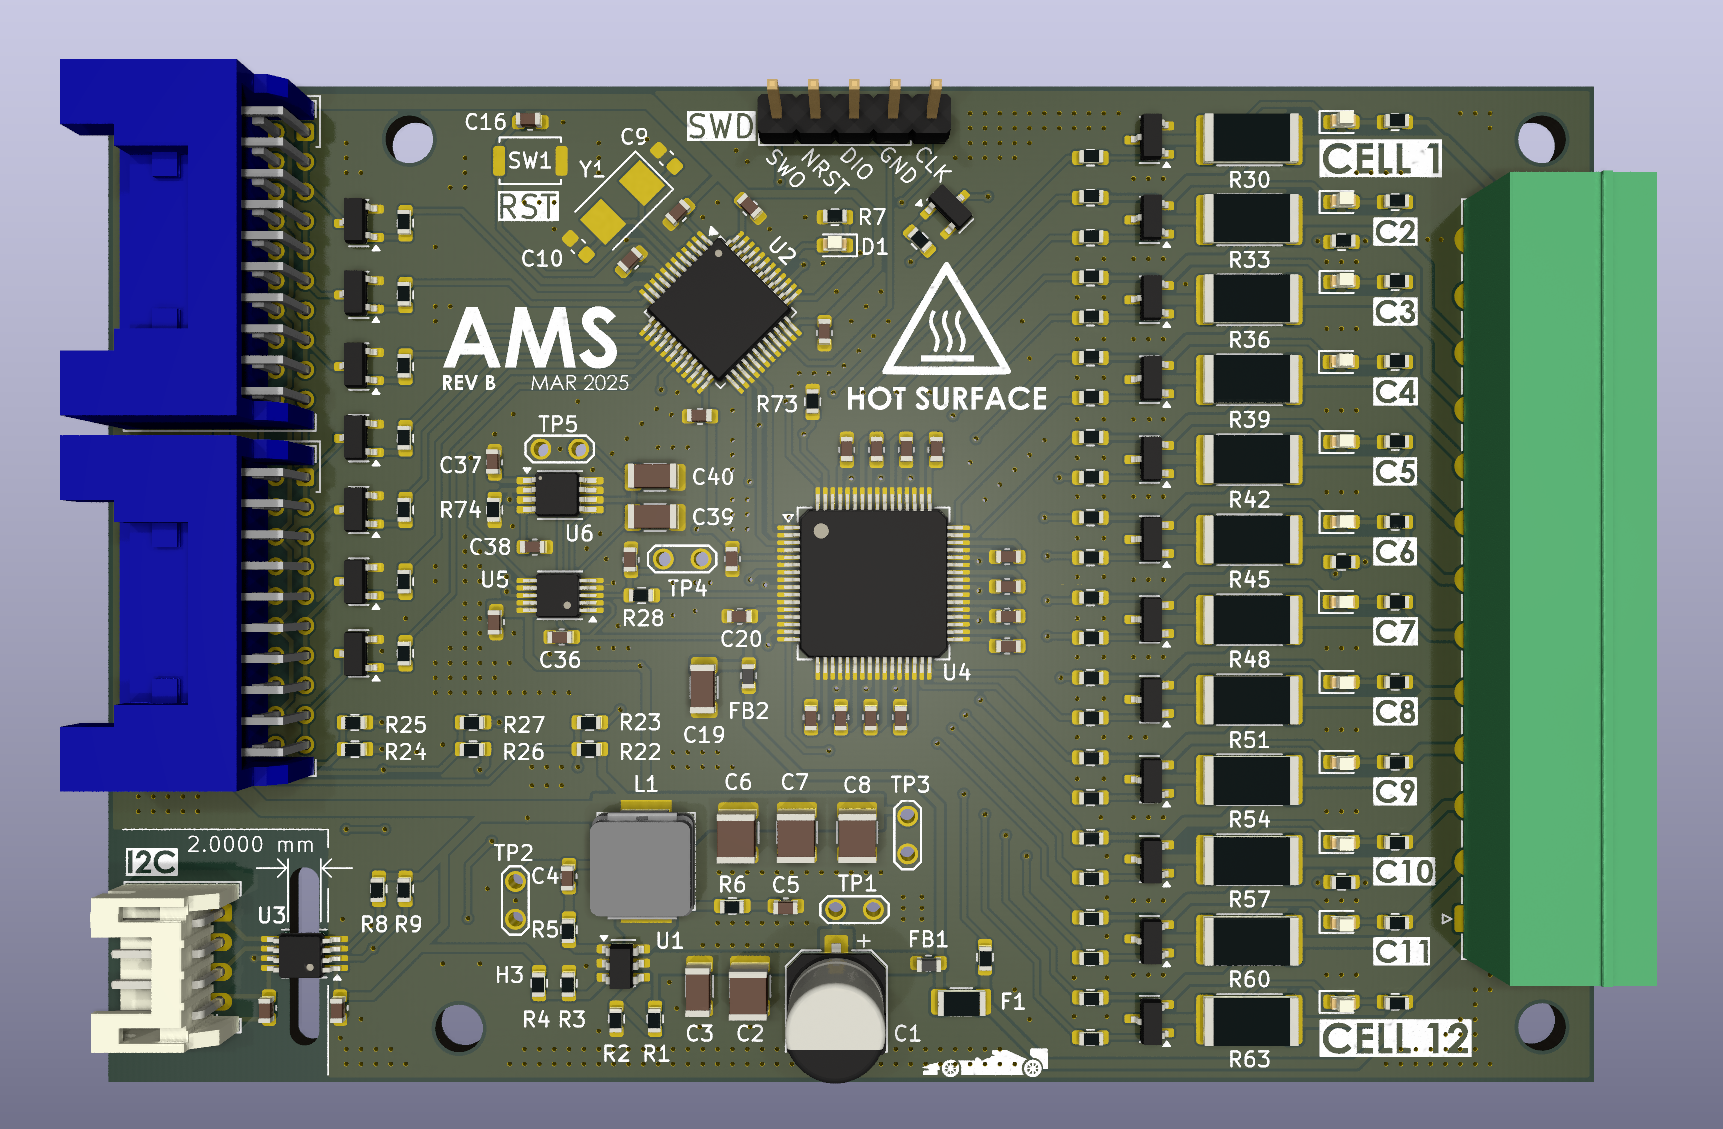
\includegraphics[width=\linewidth]{bms.png}
  \caption{Segment BMS PCB Render}
  \label{fig:bms-pcb}
\end{figure}

\subsection{Applicable Rules}
As per the FSUK 2025 rules, the BMS must:
\begin{itemize}
\item[(EV5.8.1)] Be monitoring whenever the low-voltage system or charging is active.
\item[(EV5.8.3)] Continuously measure:
  \begin{itemize}
  \item All cell voltages;
  \item The temperature of at least 30\% of all cells;
  \item The total tractive system current.
  \end{itemize}
\item[(EV5.8.7)] Switch off the tractive system via the shutdown circuit if critical voltage, temperature, or current values are reached and are persistent for more than:
  \begin{itemize}
  \item 500 ms for voltage and current values;
  \item 1 s for temperature values.
  \end{itemize}
\item[(EV5.8.10)] Fail-safe.
  In particular, all signals are system critical signals, meaning the loss of any measurement signal must result in an opened shutdown circuit.
\item[(EV5.8.11)] Have individually disconnectable current sensors, temperature sensors, and cell voltage taps.
\item[(EV5.8.12)] Be able to display all measured values at any time.
\end{itemize}

In general, the BMS does not need to concern itself with rule EV1.2.2:
\begin{displayquote}
  High Current Path -- any path of a TS circuitry that, during normal operation, carries more than 1A.
\end{displayquote}
Since no significant current, other than cell balance current which is under one amp, flows through the BMS.
In particular, this means that the BMS connections are not required to be positively locking.

\subsection{High-Level Design}
Although the accumulator is physically divided into five segments, from the perspective of the BMS, there are ten segments.
This design choice was made for two primary reasons:
\begin{enumerate}[label=(\arabic*)]
\item Each distributed BMS board is limited to handling a maximum of 50 volts, making the system both safer to work with and more practical for testing and development.
\item By dividing the accumulator into ten segments, each BMS board is responsible for monitoring just 12 series cells, which is more practical compared to handling 24 cells per board.
\end{enumerate}

Each of these ten segments is managed by a distributed segment board, all of which are connected to a master BMS via an isolated \iic{} bus.
The segment boards operate in a passive manner, responding to requests from the master BMS to perform a measurement of all cell voltages and temperatures.
When the low-voltage system is active, the master BMS polls each segment board at a regular interval.
In the event of a segment BMS failure, \iic{} communication would be lost, but the system fails safe with the master BMS opening the shutdown circuit.

Charging control is managed by the master BMS through a GPIO output.
During charging, the segment boards enter a continuous measurement mode, which acts mostly autonomously.
In this mode, the cell balancing algorithm is enabled.
A periodic heartbeat message is sent from the master BMS to each distributed board to confirm that charging is still active, and a response from each segment BMS to the master BMS confirms that the cell voltages and temperatures are still within safe limits.

Current measurement is also performed by the master BMS, through the use of Hall-effect current sensors which measure the total tractive system current.
A connection to the car's CAN bus allows measurement logging and configuration of the BMS.
This CAN connection is non-critical, since the shutdown mechanism is implemented through a dedicated digital output.

\subsection{Segment-Level Design}
This section covers the distributed segment design of the BMS.
Cell voltage taps are connected via a pluggable terminal block.
Cell voltage measurements are provided by three main components:
\begin{itemize}
\item The MAX14920 12-cell measurement analog frontend
\item The MAX11163 16-bit SAR ADC
\item The REF6145 high-precision 4.5 volt reference
\end{itemize}
This selection of components allows for sub-millivolt cell voltage measurement accuracy.

The microcontroller used is the STM32F103.
Its main job is to control both the analog frontend and ADC via SPI, and communicate to the master BMS over \iic{}.
A buck converter steps-down the whole segment voltage (44 volts nominal; 50 volts maximum) to 3.3 volts to power the microcontroller and logic components of the analog frontend and ADC.

\iic{} isolation is provided by the ADuM1252 ultra-low power bidirectional \iic{} isolator IC.
This IC provides strong galvanic isolation, and allows for hot-plugging a BMS onto an active bus.

Each 4p cell set in the 12s series string has a balancer.
This is a small circuit controllable by software which bleeds off cell energy as heat during charging if cell voltages start to become unbalanced.

\begin{figure}[H]
  \centering
  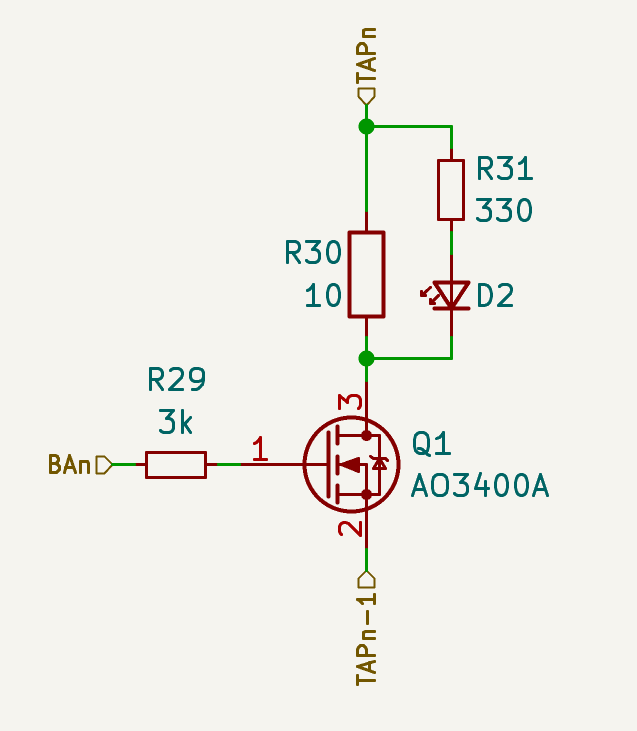
\includegraphics[width=0.5\linewidth]{balance.png}
  \caption{Cell Balance Circuit}
  \label{fig:bms-balance-circuit}
\end{figure}

The balance circuit consists of a high-power 10 ohm resistor which is shunted across cell N and cell N-1 by the MOSFET when the digital balance signal is high.
This balance signal is provided by the MAX14920 analog frontend IC, which has an internal pull-down so no external gate-source resistor is necessary.
An LED is also present to visually indicate when balancing of each cell is active.
A value of 10 ohms was chosen to achieve a balance current of about 400 mA, which results in around 100 mA per cell.

The BMS provides cell temperature monitoring via simple NTC thermistors.
Up to 20 external thermistors can be connected, which is more than the 15 minimum required by rule EV5.8.3 for our 12s4p configuration.
Additionally, there are three onboard thermistors spaced evenly around the balance section in order to monitor the temperature of the bleed resistors.

\begin{figure}[H]
  \centering
  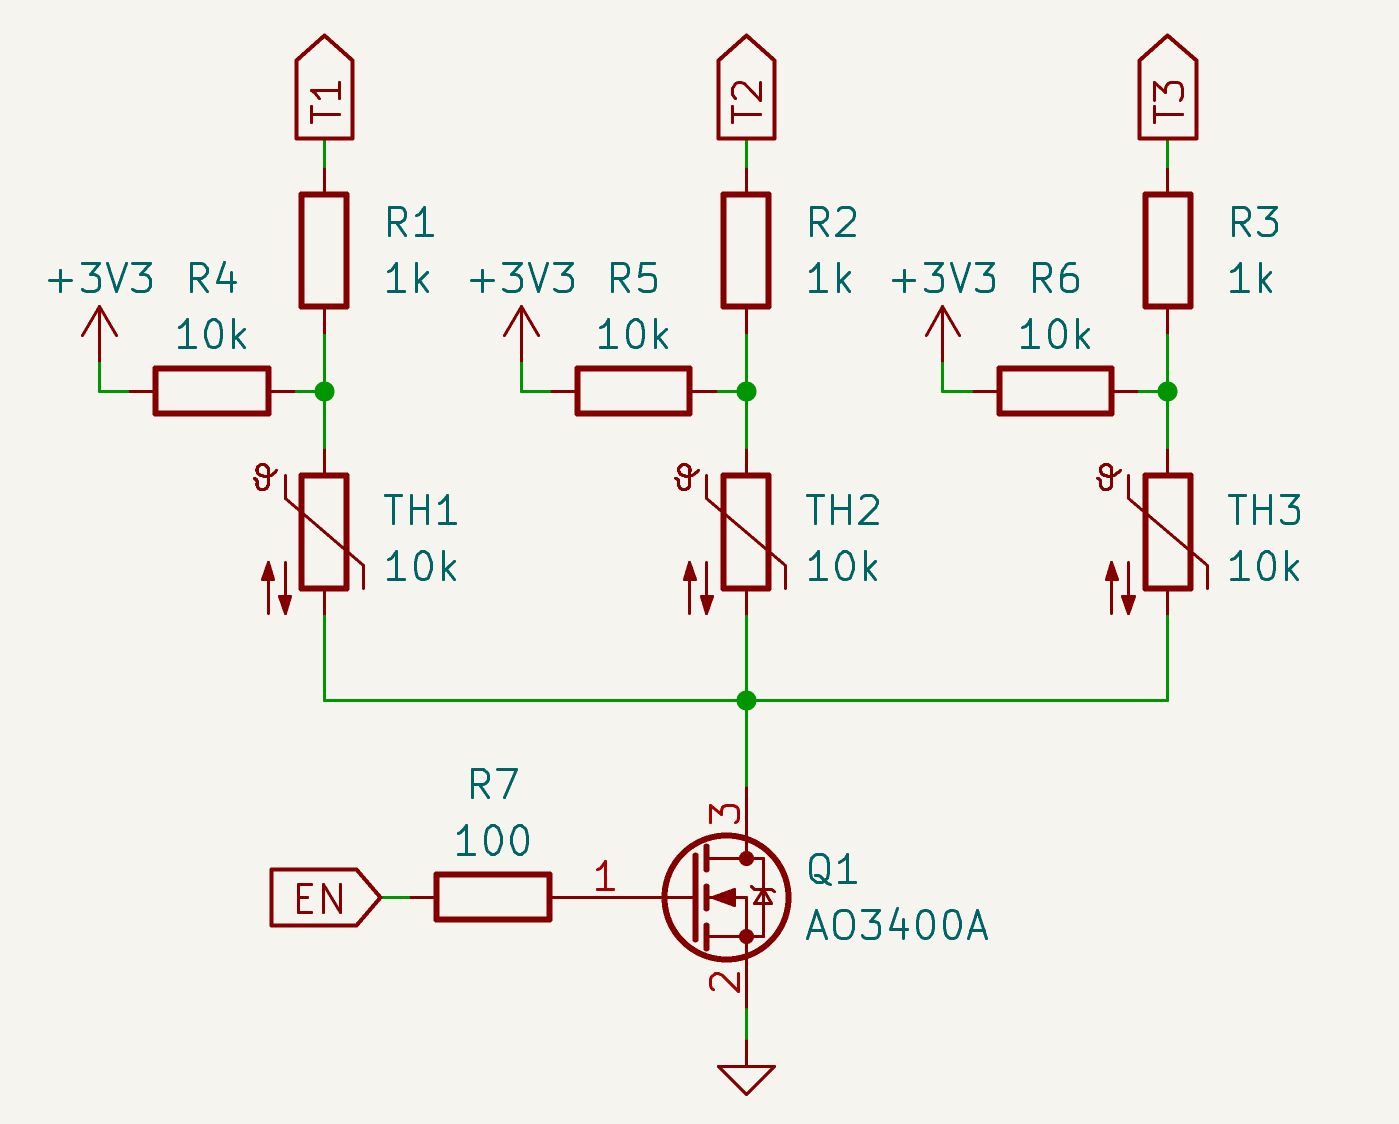
\includegraphics[width=\linewidth]{thermistor.png}
  \caption{Equivalent Thermistor Circuit}
  \label{fig:bms-thermistor-circuit}
\end{figure}

The above figure shows the equivalent schematic of the thermistor connections.
The thermistors are arranged in groups of three, with each group being switchable by the Q1 MOSFET.
T1-T3 are the auxillary single-ended analog inputs of the MAX14920 analog frontend IC, protected by the 1k series resistors.
R4-R6 are pull-up resistors forming a potential divider with the thermistors.
Q1 has a gate resistor and is driven by the main STM32F103 microcontroller.

Importantly, the precision reference used for cell voltage measurement is not used for temperature measurement, but rather the regular 3V3 power rail.
This was done to reduce complexity since the accuracy of the thermistor measurements is not super critical, and the nonlinearities and tolerances from the thermistors themselves will result in more error than the ADC reference voltage.

As both the cell tap and thermistor connections are system critical, the system must fail safe in the event of either an open or a short circuit.
The following table describes the possible scenarios.

\begin{table}[H]
  \centering
  \begin{tabular}{|p{0.3\linewidth}|p{0.7\linewidth}|}
    \hline
    \textbf{Failure} & \textbf{Mitigation} \\
    \hline
    Cell tap disconnected & TBD \\
    \hline
    Cell tap shorted to another cell/ground & The cell voltage would become out of range for measurement, which would be detected.
                                              In addition, a large current may flow causing the individual cell fuse to blow, which would effectively look like a disconnected cell tap to the BMS (see above). \\
    \hline
    Thermistor disconnected or shorted to supply voltage & The signal would read 3.3 volts, which is above the plausible range. \\
    \hline
    Thermistor shorted to ground & The signal would read 0 volts, which is below the plausible range. \\
    \hline
  \end{tabular}
  \caption{Segment BMS SCS Compliance}
  \label{tbl:segment-bms-scs-compliance}
\end{table}

\subsection{Current Unknowns}
\begin{itemize}
\item How to power the main BMS board.
\item How EV3.2.5 fits in with the current measurement of the master BMS.
\end{itemize}

\begin{versionhistory}
  \vhEntry{1.0}{06/04/2025}{OS}{Initial version}
\end{versionhistory}

\end{document}
